\documentclass[tikz, border=2pt]{standalone}
\usepackage[utf8]{inputenc}
\usepackage{tikz}
\usetikzlibrary{bayesnet}

% \title{shift_multi_source}
% \author{Vishal Ghoniya}
% \date{July 2022}

\begin{document}
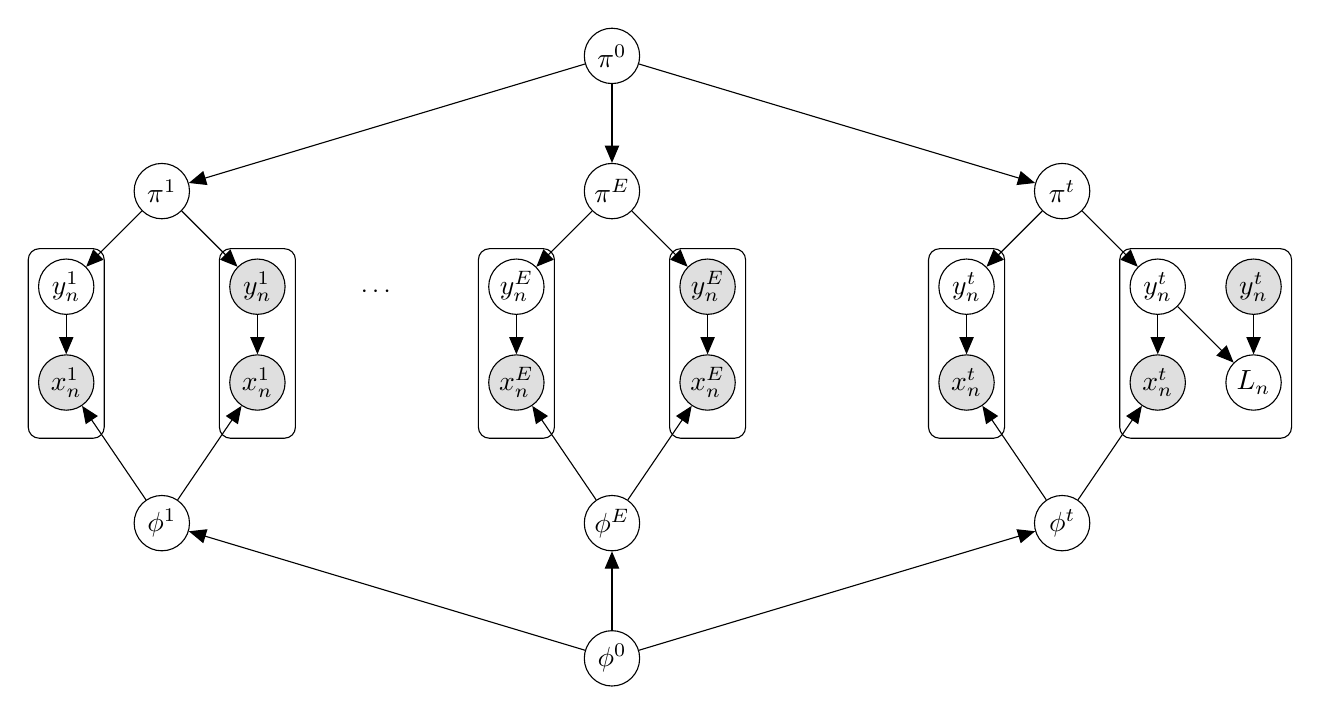
\begin{tikzpicture}[font={\small}]
    \node [latent, ] (pi_0) {$\pi^0$};
        \node [latent,  below=1cm of pi_0] (pi_e) {$\pi^E$};
        \node [latent, left=5cm of pi_e] (pi_1) {$\pi^1$};
        \node [latent,  right=5cm of pi_e] (pi_t) {$\pi^t$};
        \edge{pi_0}{pi_1, pi_e, pi_t};
    \node [latent, below left=1cm of pi_1] (y_n1l) {$y_n^1$};
    \node [obs, below=0.5cm of y_n1l] (x_n1l) {$x_n^1$};
    \plate {}{(y_n1l)(x_n1l)}{};
    
    \node [obs, below right=1cm of pi_1] (y_n1o) {$y_n^1$};
    \node[obs, below=0.5cm of y_n1o] (x_n1o) {$x_n^1$};
    \plate{}{(y_n1o)(x_n1o)}{};
    
    \edge{pi_1}{y_n1l, y_n1o};
    \edge{y_n1l}{x_n1l};
    \edge{y_n1o}{x_n1o};
    \draw (-3,-3) node {$\cdots$};
    
    \node [latent, below left=1cm of pi_e] (y_nel) {$y_n^E$};
    \node [obs, below right=1cm of pi_e] (y_neo) {$y_n^E$};
    \edge{pi_e}{y_nel, y_neo};
    \node [obs, below=0.5cm of y_nel] (x_nel) {$x_n^E$};
    \node [obs, below=0.5cm of y_neo] (x_neo) {$x_n^E$};
    \edge{y_nel}{x_nel};
    \edge{y_neo}{x_neo};
    \plate{}{(y_nel)(x_nel)}{};
    \plate{}{(y_neo)(x_neo)}{};
    
    \node [latent, below left=1cm of pi_t] (y_nt) {$y_n^t$};
    \node [latent, below right=1cm of pi_t] (y_nt1) {$y_n^t$};
    \edge{pi_t}{y_nt, y_nt1};
    \node [obs, right=0.5cm of y_nt1] (y_nto) {$y_n^t$};
    \node[obs, below=0.5cm of y_nt] (x_nt) {$x_n^t$};
    \edge{y_nt}{x_nt};
    \plate{}{(y_nt)(x_nt)}{}
    \node[latent,  below=0.5cm of y_nto] (ln) {$L_n$};
    \edge{y_nt1, y_nto}{ln};
    \node[obs, below=0.5cm of y_nt1] (x_nt1) {$x_n^t$};
    \edge{y_nt1}{x_nt1};
    \plate{}{(y_nt1)(y_nto)(x_nt1)}{};
    
    % draw without a circle
    %    \node[circle, draw=black!0, below=3.5cm of pi_1] (phi_1) {$\phi^1$};
    
    \node[latent,  below=3.5cm of pi_1] (phi_1) {$\phi^1$};
    \node[latent,  below=3.5cm of pi_e] (phi_E) {$\phi^E$};
    \node[latent, below=3.5cm of pi_t] (phi_t) {$\phi^t$};
    \edge{phi_1}{x_n1l, x_n1o};
    \edge{phi_E}{x_nel, x_neo};
    \edge{phi_t}{x_nt, x_nt1};

    \node[latent,  below=1cm of phi_E] (phi_0) {$\phi^0$};
    \edge{phi_0}{phi_1, phi_E, phi_t};
    
\end{tikzpicture}

\end{document}
